


\tikzset{every picture/.style={line width=0.75pt}} %set default line width to 0.75pt        

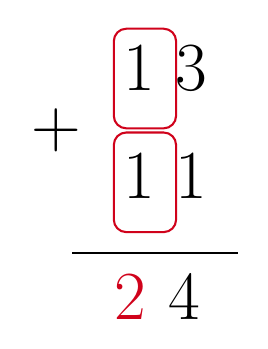
\begin{tikzpicture}[x=0.75pt,y=0.75pt,yscale=-1,xscale=1]
%uncomment if require: \path (0,300); %set diagram left start at 0, and has height of 300

%Straight Lines [id:da487957330965736] 
\draw    (230,148) -- (310,148) ;
%Rounded Rect [id:dp6610606653132355] 
\draw  [color={rgb, 255:red, 208; green, 2; blue, 27 }  ,draw opacity=1 ] (250,46) .. controls (250,42.69) and (252.69,40) .. (256,40) -- (274,40) .. controls (277.31,40) and (280,42.69) .. (280,46) -- (280,82) .. controls (280,85.31) and (277.31,88) .. (274,88) -- (256,88) .. controls (252.69,88) and (250,85.31) .. (250,82) -- cycle ;
%Rounded Rect [id:dp30531342140045525] 
\draw  [color={rgb, 255:red, 208; green, 2; blue, 27 }  ,draw opacity=1 ] (250,96) .. controls (250,92.69) and (252.69,90) .. (256,90) -- (274,90) .. controls (277.31,90) and (280,92.69) .. (280,96) -- (280,132) .. controls (280,135.31) and (277.31,138) .. (274,138) -- (256,138) .. controls (252.69,138) and (250,135.31) .. (250,132) -- cycle ;

% Text Node
\draw (253,47) node [anchor=north west][inner sep=0.75pt]  [font=\Huge] [align=left] {1 3};
% Text Node
\draw (253,99) node [anchor=north west][inner sep=0.75pt]  [font=\Huge] [align=left] {1 1};
% Text Node
\draw (209,77) node [anchor=north west][inner sep=0.75pt]  [font=\Huge] [align=left] {+};
% Text Node
\draw (249,157) node [anchor=north west][inner sep=0.75pt]  [font=\Huge,color={rgb, 255:red, 208; green, 2; blue, 27 }  ,opacity=1 ] [align=left] {2};
% Text Node
\draw (275,157) node [anchor=north west][inner sep=0.75pt]  [font=\Huge,color={rgb, 255:red, 0; green, 0; blue, 0 }  ,opacity=1 ] [align=left] {4};


\end{tikzpicture}
